\section{Results of basic part}
\subsection{Correctness}
All indexes  of the basic part passed all levels of the correctness test.

\subsection{Time complexity}
\subsubsection{Indexing time}
Figure \ref{fig:BPindextime2}, \ref{fig:BPindextime3}, \ref{fig:BPindextime45} shows the indexing time for index 2,3,4 and 5. Notice that the y-axis varies from plot to plot. Figure \ref{fig:BPindextime2345} shows all indexes compared to each other on a log-transformed plot to compare them against each other.

\begin{figure}[H]
    \centering
    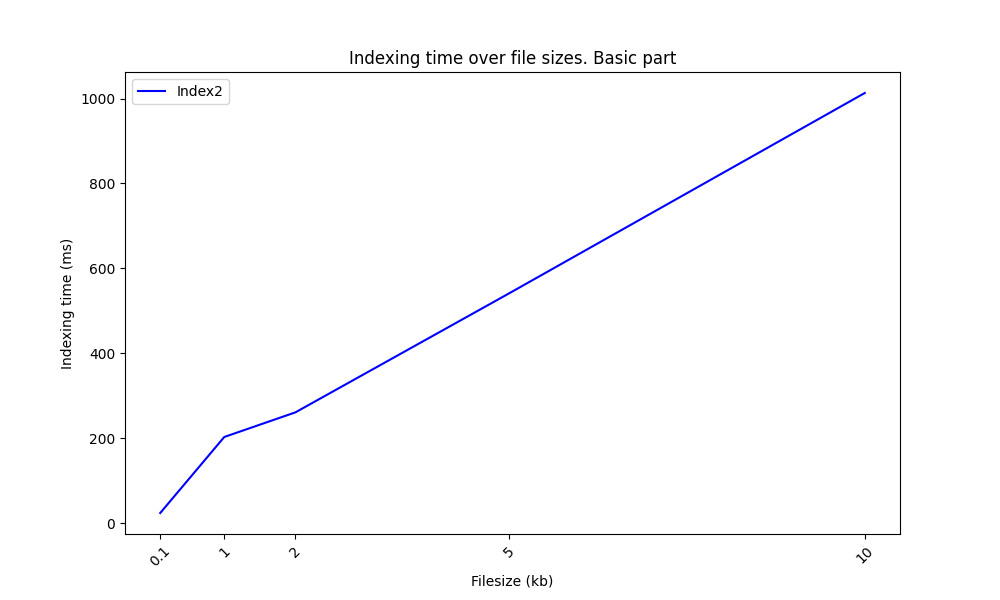
\includegraphics[width=.8\textwidth]{LaTeX/Figures/BasicPart/BPIndexing[2].png}
    \caption{Indexing time for index 2 over different filesizes}
    \label{fig:BPindextime2}
\end{figure}

\begin{figure}[H]
    \centering
    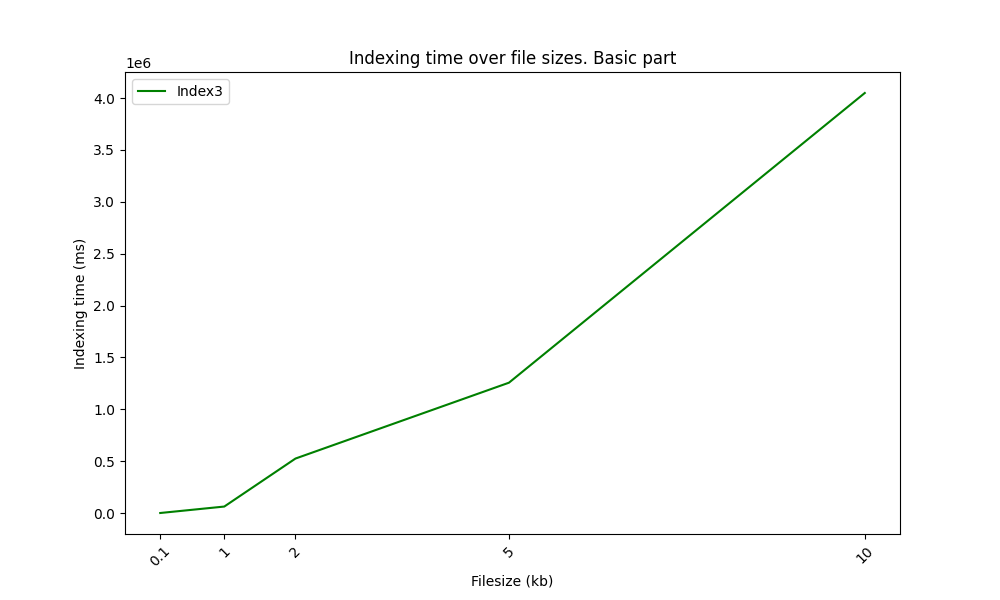
\includegraphics[width=.8\textwidth]{LaTeX/Figures/BasicPart/BPIndexing[3].png}
    \caption{Indexing time for index 2 over different filesizes}
    \label{fig:BPindextime3}
\end{figure}

\begin{figure}[H]
    \centering
    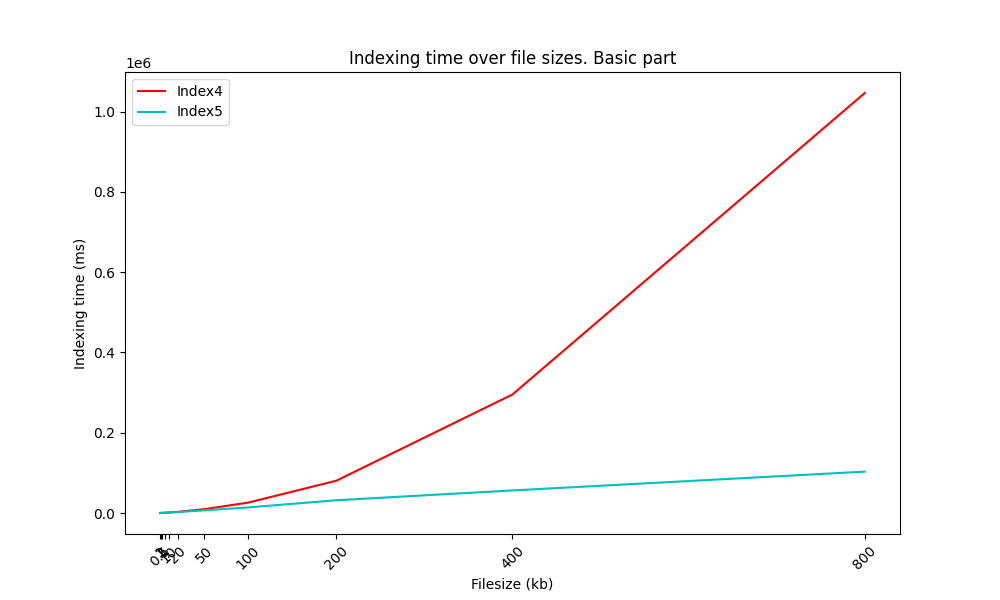
\includegraphics[width=.8\textwidth]{LaTeX/Figures/BasicPart/BPIndexing[4, 5].png}
    \caption{Indexing time for index 2 over different filesizes}
    \label{fig:BPindextime45}
\end{figure}

\begin{figure}[H]
    \centering
    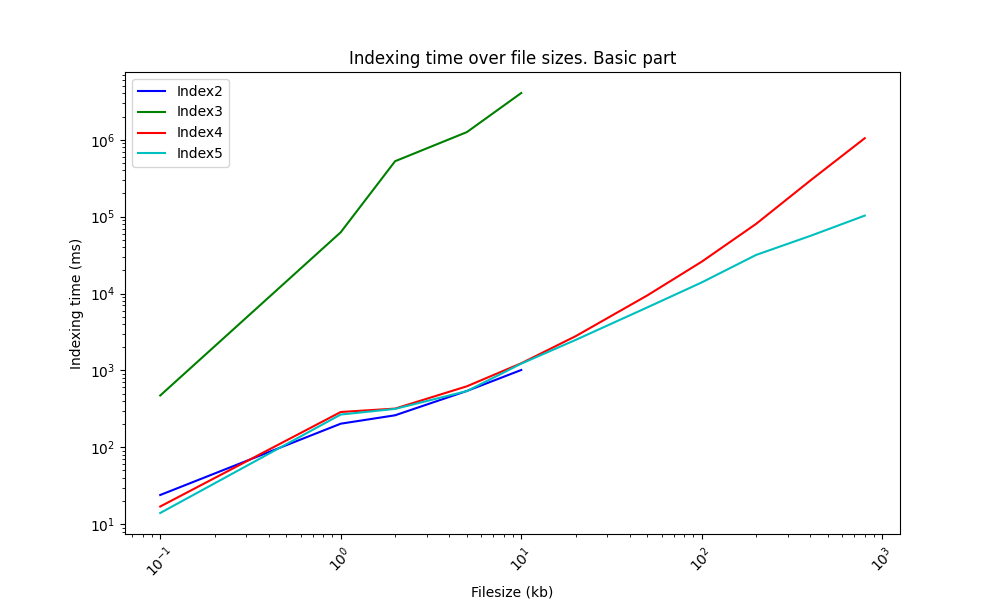
\includegraphics[width=.8\textwidth]{LaTeX/Figures/BasicPart/BPIndexing[2, 3, 4, 5].png}
    \caption{Indexing time for index 2 over different filesizes}
    \label{fig:BPindextime2345}
\end{figure}

The time complexity of indexing for index2 is analysed to be linear. This tendency is also seen in figure \ref{fig:BPindextime2}.

Index 3 is analysed to have $O(n^2)$ indexing time complexity. It is tricky to declare if figure \ref{fig:BPindextime3} shows that the indexing running time is Linear or quadratic, due to the lack of data points. No additional data points for the indexing time of index3 were provided, as this was very time-consuming. In figure \ref{fig:BPindextime2345} index3 is compared to the other indexes of the Basic Part. The figure illustrates how poorly index3 performs compared to the other indexes. The architecture of the data structure of index3 was however never predicted to be an effective design compared to hashmaps.  

Figure \ref{fig:BPindextime45} shows that the indexing time for index 5 is linear. Index 4 is analysed to have a time complexity of $O(n^2)$ as index 4 has a static hash map where all entries at some point can be used, meaning that multiple words share the same hash key. This slows down the indexing time tremendously. In figure \ref{fig:BPindextime45}, index 5 performs much better than index4. This is due to the fact that index 5 uses a dynamic hash map. 

\subsubsection{Search time}
Figure \ref{fig:BPindextime2}, \ref{fig:BPindextime3}, shows the searching time for index 2,3,4 and 5.

\begin{figure}[H]
    \centering
    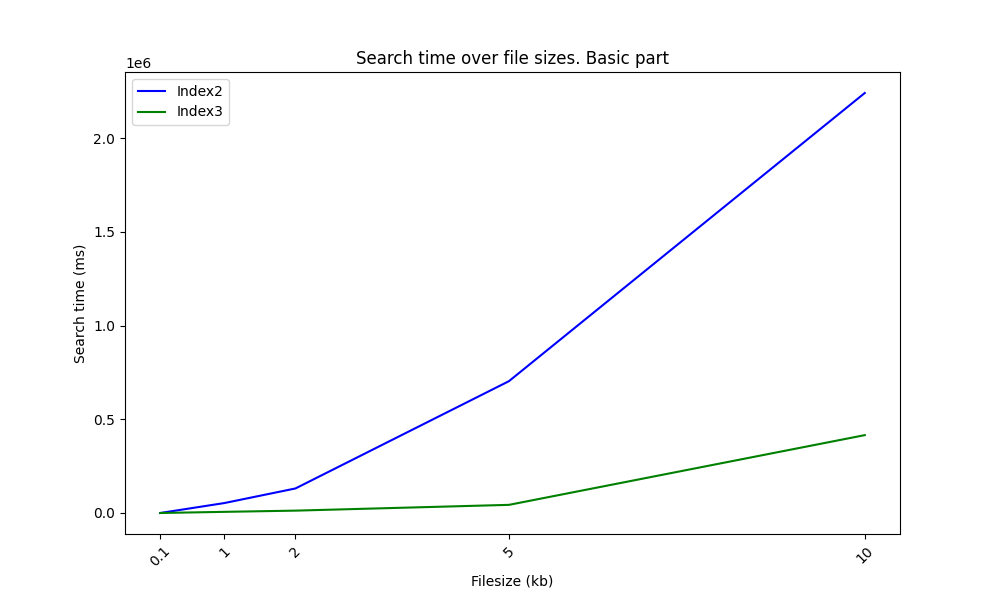
\includegraphics[width=.8\textwidth]{LaTeX/Figures/BasicPart/BPSearch[2, 3].png}
    \caption{Searching time for index2 and index3 over different filesizes}
    \label{fig:BPsearch23}
\end{figure}

\begin{figure}[H]
    \centering
    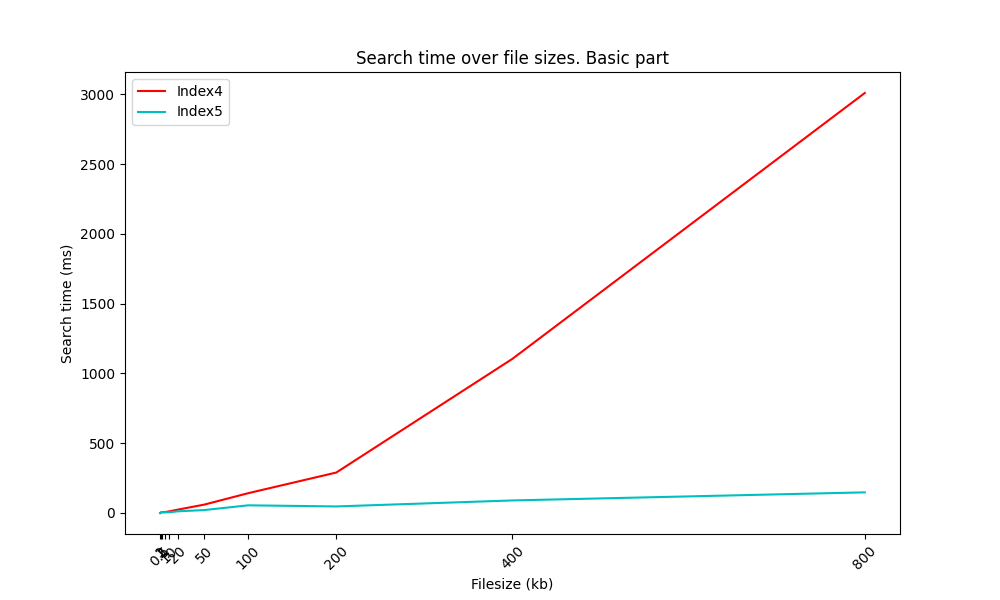
\includegraphics[width=.8\textwidth]{LaTeX/Figures/BasicPart/BPSearch[4, 5].png}
    \caption{Searching time for index4 and index 5 over different filesizes}
    \label{fig:BPsearch45}
\end{figure}

Index2 is analysed to have a searchtime complexcity of $O(n)$ while index3 has a searchtime complexcity $O(u)$, and is is therefor predicted that index 3 will perform better as $u\leq n$. This is also the tendency seen in \ref{fig:BPsearch23}.

Figure \ref{fig:BPsearch45} shows that the indexing time for index 5 is constant. Index 4 is analysed to have a time complexity of $O(n)$ as multiple words share the same hash key, which it then has to search through linearly. This slows down the searhing time tremendously. In figure \ref{fig:BPsearch23}, it is seen that index5 searches in constant time, which once again shows the benefits of a dynamic hashmap.  




